\documentclass[tikz,border=10pt]{standalone}
\usetikzlibrary{patterns,decorations.pathreplacing}
\usepackage{amsmath,amssymb}
\usepackage{pgfplots}
\pgfplotsset{compat=1.18}
\usepgfplotslibrary{fillbetween}
\begin{document}
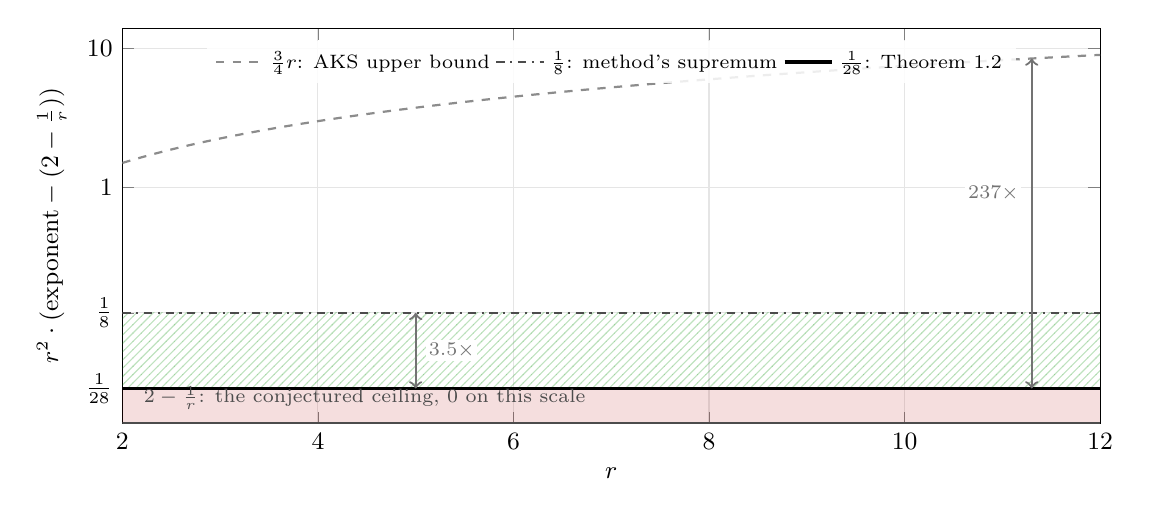
\begin{tikzpicture}
\begin{semilogyaxis}[
  width=14cm, height=6.6cm,
  xlabel={$r$},
  ylabel={$r^2\cdot(\text{exponent}-(2-\tfrac1r))$},
  xmin=2, xmax=12, xtick={2,4,6,8,10,12},
  ymin=0.02, ymax=14,
  ytick={0.0357142857,0.125,1,10},
  yticklabels={$\tfrac1{28}$,$\tfrac18$,$1$,$10$},
  grid=major, grid style={black!10},
  every axis label/.append style={font=\small},
  tick label style={font=\small},
  legend style={font=\scriptsize, draw=none, fill=white, fill opacity=0.85,
    text opacity=1, at={(0.5,0.97)}, anchor=north},
  legend columns=3, legend cell align=left]

\addplot[name path=aks, domain=2:12, samples=100, thick, black!45, dashed]
  {0.75*x};
\addlegendentry{$\tfrac34r$: AKS upper bound}
\addplot[name path=sup, domain=2:12, samples=2, thick, black!70, dash dot]
  {0.125};
\addlegendentry{$\tfrac18$: method's supremum}
\addplot[name path=ours, domain=2:12, samples=2, very thick] {1/28};
\addlegendentry{$\tfrac1{28}$: Theorem 1.2}

\path[name path=floor] (axis cs:2,0.02) -- (axis cs:12,0.02);
% refuted: above the conjectured ceiling, proved reachable for every r
\addplot[red!70!black, fill opacity=0.13, forget plot]
  fill between[of=floor and ours];
% open to the method
\addplot[pattern=north east lines, pattern color=green!55!black,
  opacity=0.25, forget plot] fill between[of=ours and sup];

% the conjectured ceiling is 0 here, i.e. the floor of a log axis
\draw[very thick, black!70] (axis cs:2,0.02) -- (axis cs:12,0.02);
\node[font=\scriptsize, anchor=south west, black!70]
  at (axis cs:2.12,0.0215) {$2-\tfrac1r$: the conjectured ceiling, $0$ on this scale};

% the two gaps, read off as ratios
\draw[<->, thick, black!55] (axis cs:11.3,0.0357) -- (axis cs:11.3,8.475);
\node[font=\scriptsize, anchor=east, black!55, fill=white, inner sep=1pt]
  at (axis cs:11.2,0.9) {$237\times$};
\draw[<->, thick, black!55] (axis cs:5,0.0357) -- (axis cs:5,0.125);
\node[font=\scriptsize, anchor=west, black!55, fill=white, inner sep=1pt]
  at (axis cs:5.1,0.067) {$3.5\times$};
\end{semilogyaxis}
\end{tikzpicture}
\end{document}
